\chapter{TOWARDS HIGH DIMENSION}
\label{chap:highdor}
\ifpdf
    \graphicspath{{BipedWalk/HiDofFigs/PNG/}{HiDof/HiDofFigs/PDF/}{HiDof/HiDofFigs/}}
\else
    \graphicspath{{HiDof/HiDofFigs/EPS/}{HiDof/HiDofFigs/}}
\fi
\section{Introduction}
\subsection*{Passivity}
High DOF is key challenging in motion synthesis.
In our research, we partly solved the problem.
For our walking model, when it walks down the slop, all the dof is uncontrolled.
how many dof the walker have doesn't matter.
Even controlled with neural oscillator, only one dof is controlled, 
Even when transformation controller is added, all the dof are controlled, but the matter will not result in nondeterministic problem.
For our model, even the dof is not so huge, we have solved extra dof problem completely.

the question arise for model of high degree system, the question is whether the method we developed is applicable for large dof characters.


for our walking and stance example, the question is how the torso should be added, the foot, the side sway and yaw motion, and for system like fish and snake and worm,
they have infinite number dof 

our idea is for different model, 
we should take different measures, 
\begin{itemize}

\HiItem{Neglectable}
for some dof can be neglected for they will have little effects on the qualitative property, 
we can simulate them a different mechanical model, our motion control method don't have to be changed.
because the qualitative property and symmetry is kept.
\HiItem{Symmetry Reduction}
For some DOF,like rotation or pos, the extra dof will have not effects on the dof or the effects can be transformed the dynamic system into transformed version of the original system, such Dofs can be reduced.
\HiItem{Mechanical Coupling}
For some high dof system, we can treat them like a coupled mechanical oscillator, the can only focus on one oscillator.
\HiItem{mimic}
all the three method above are based the effects of dof are not equal, for system that all the dofs are the some, such method will not work.
For dof with similar effects, we can propose a different method, the system is divided into several equal component, we only calculate one component, other mimic the strategy of one.
\end{itemize} 

\section{neglectable}
Although biological mechanical structure is of high degree of freedom, many dof will not have effects on the topology or symmetrical properties.
For the walking example,marcke raiber\citet{Raibert1986} point out walking is the same as a ball rolling down a slope while running is ball bounding down a slope.


we can have system from low dof to high dof as the following picture.
\begin{itemize}
\HiItem{Rimless Wheel}
\HiItem{Compass Gait}
\HiItem{Arch Foot}
\HiItem{Our Model}
\end{itemize}


\begin{figure}[!htbp]
  \begin{center}
    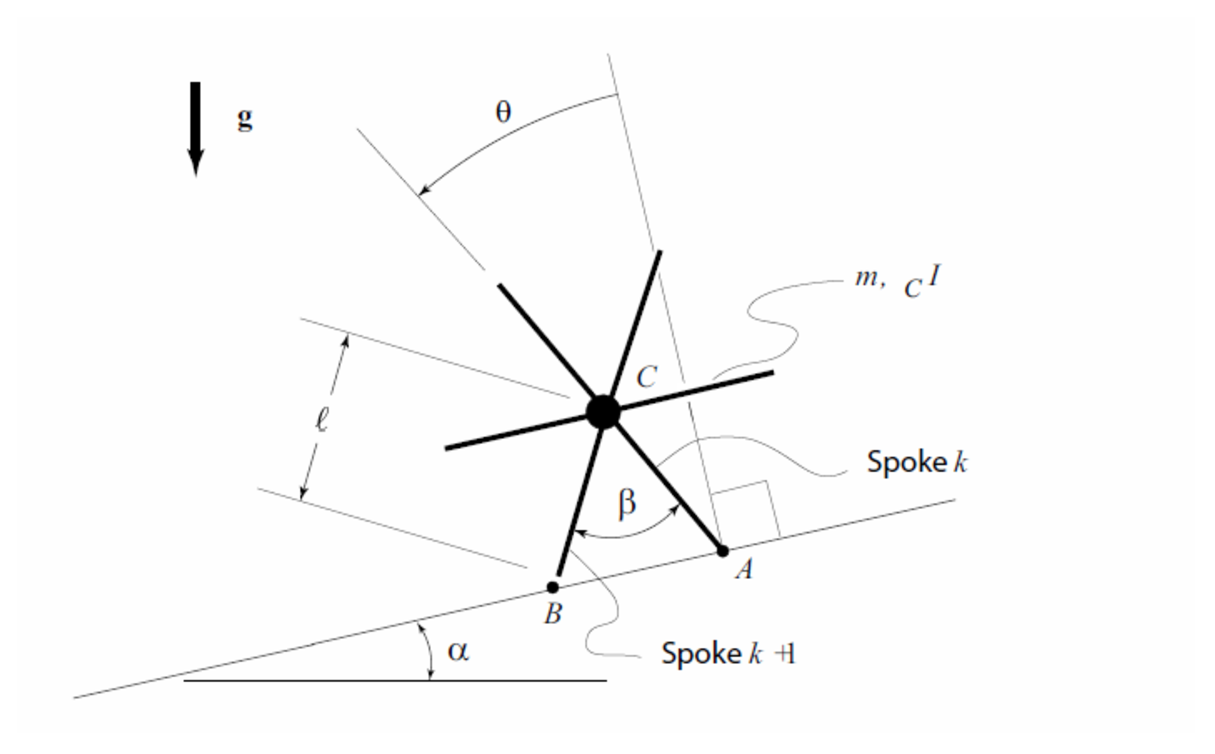
\includegraphics[width=0.7\textwidth]{rimlesswheel}
    \caption{Rimless Wheel}
    \label{fig:rimlesswheel}
\end{center}
\end{figure}


\begin{figure}[!htbp]
  \begin{center}
      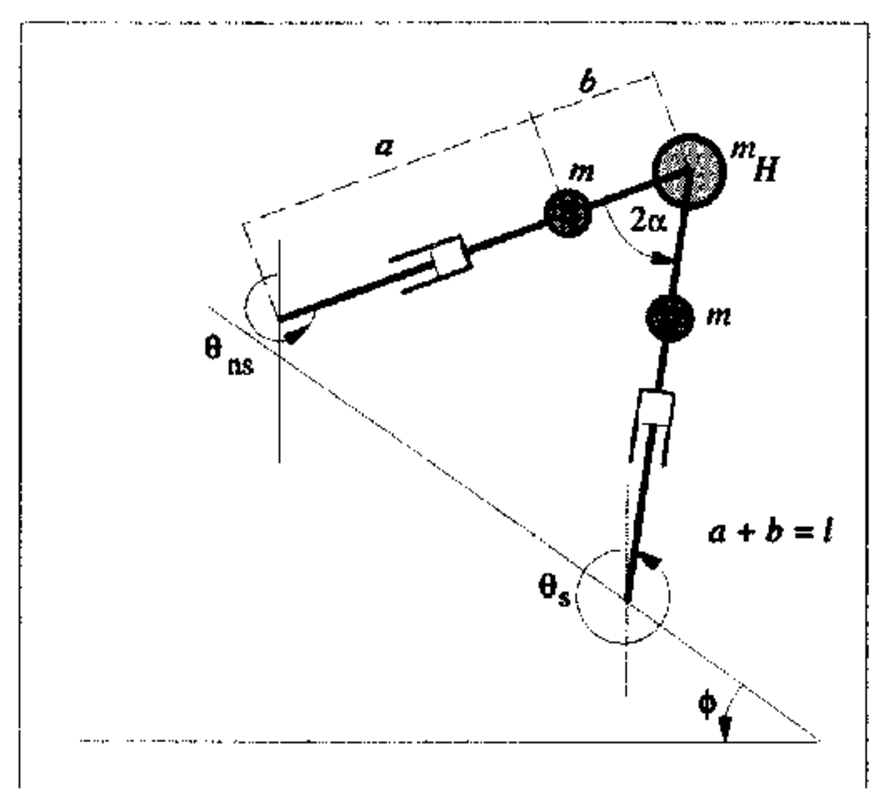
\includegraphics[width=0.7\textwidth]{compassgait}
    \caption{Compass Gait}
    \label{fig:compassgait}
\end{center}
\end{figure}


\begin{figure}[!htbp]
  \begin{center}
      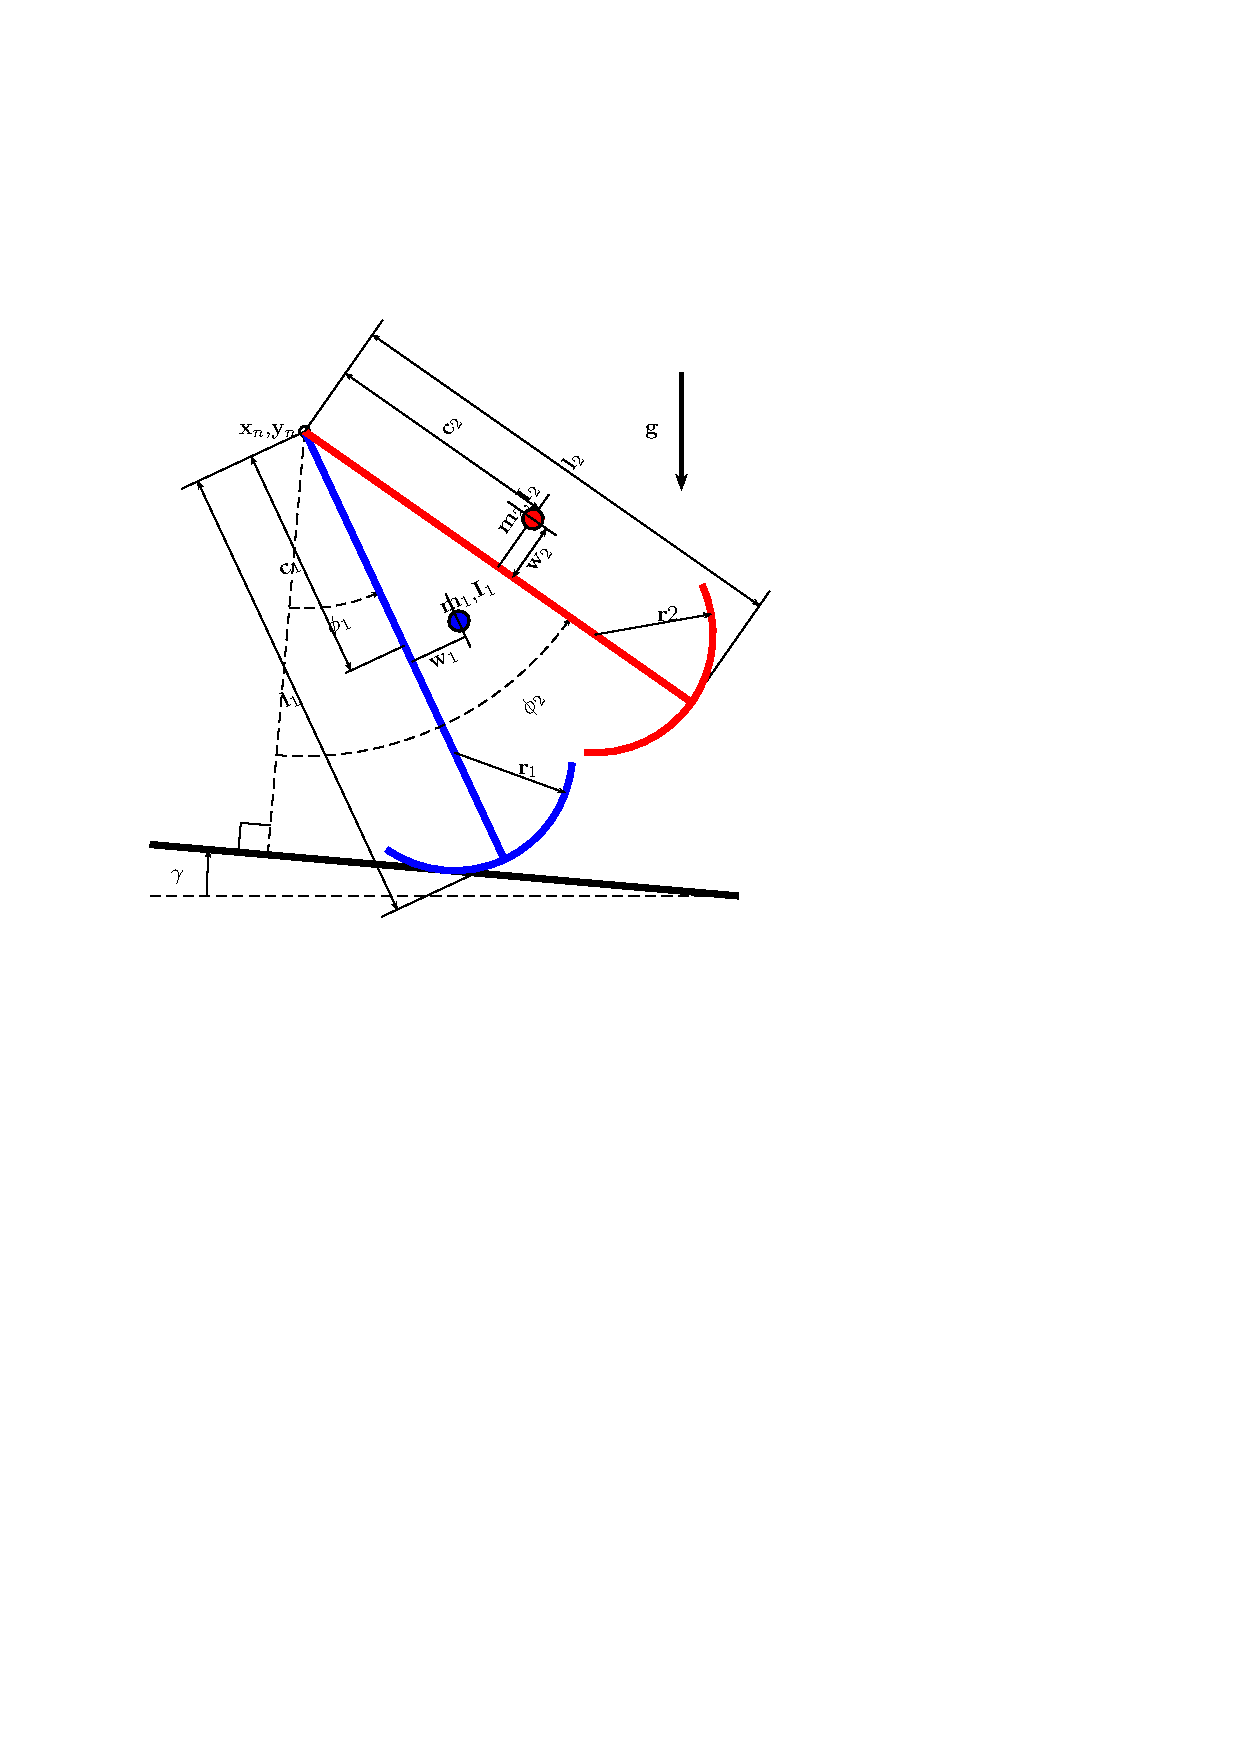
\includegraphics[width=0.7\textwidth]{rollfoot}
    \caption{Compass Gait}
    \label{fig:compassgait}
\end{center}
\end{figure}


compare with our knee walker, all the four models are different but they share the same topology structure and the following three the limit circle shape is very similar.
Thus we can say, the include or knee will not affect the qualitative properties.


And all the four system, can apply the same kind of symmetry group.


This idea may be understand through the perturbation or averaging theory.

In theory all the manifolds share the shape of torus.

if the motion is relatively small,

the dynamics can be approximate as a low dimensional cycle.

as show in Figure.

\begin{figure}[!htbp]
  \begin{center}
      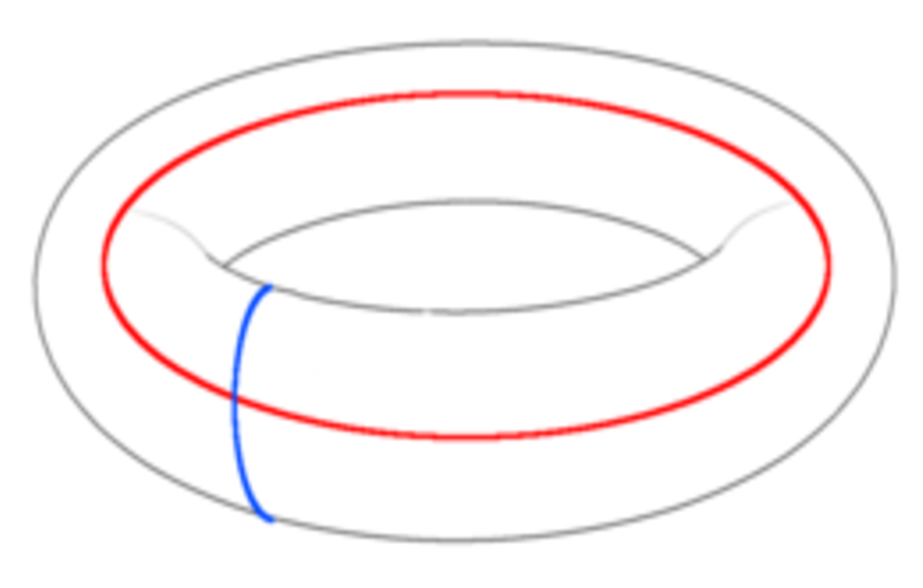
\includegraphics[width=0.7\textwidth]{Torus}
    \caption{Approximate with Torus with a Circle}
    \label{fig:approximate}
\end{center}
\end{figure}


Following this idea, although not implemented in this research, more dofs like foot may also possible.
But that's just an extra level of complexity, without modifying the principles. 
\section{Symmetry Reduction}
Some dof will result in a different motion, but such kind of motion will have not qualitative effects.
An example is the side sway motion.

the side and front plane is show in picture.
The side sway effects can be seen can be decoupled for spaghetti function.


For different rotation, will not affect the dynamics on the sphatetal plane.
thus can be neglected.

This method is we can project the gravity in the spagetta plane,
then we see, the way function is just an uniform of minimizing the gravity,
which is the same as speed action.

\begin{figure}[!htbp]
  \begin{center}
      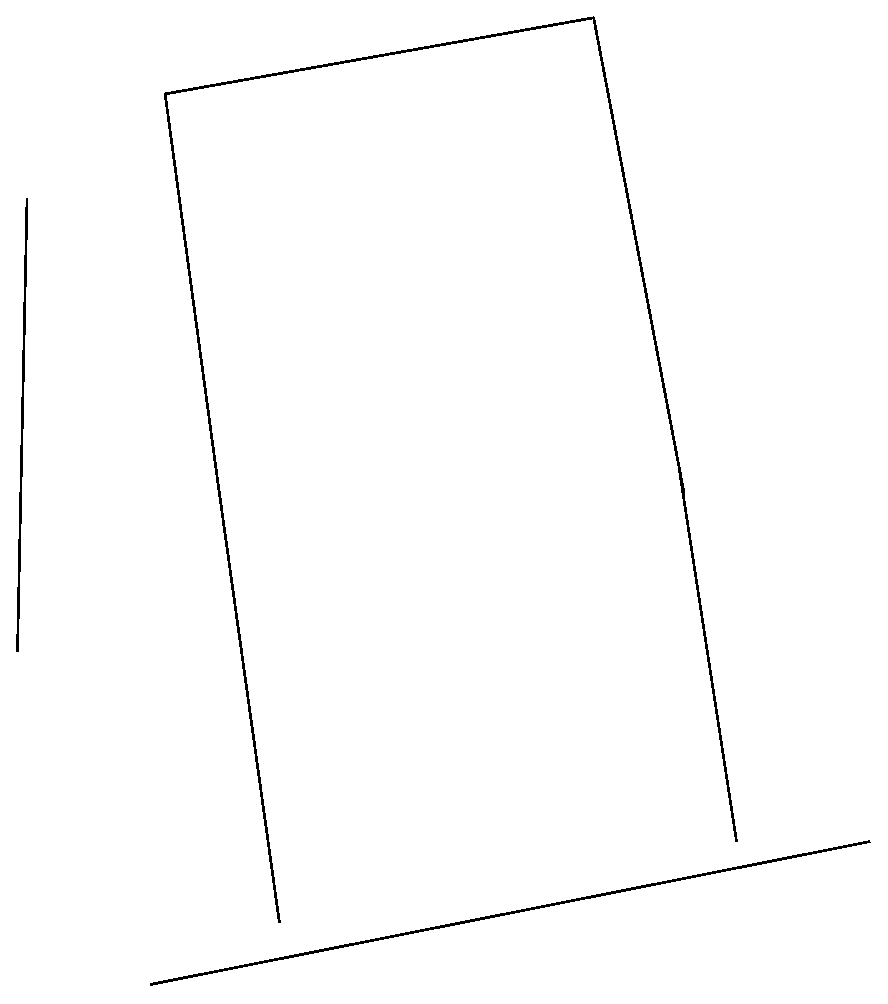
\includegraphics[width=0.7\textwidth]{Sidesway}
    \caption{Sideway}
    \label{fig:sidesway}
\end{center}
\end{figure}


we can project the sideway effects on the sphettal plane. the force is $N'=cos(\alpha)N$
this will the same as applying speed action.
With lie group operator such dof can be totally ignored.


if we consider the difference in heel strike phase,
the limit circle becomes more a bit noisy, but qualitative properties are maintained.

\section{Mechanical Coupling}
Some mechanical system can be treated as connecting many different simple components together.
the different parts of motion formed mechanical entrainment.
if a mechanical system is model like
\[
\dot{\state}=F(\state)
\]
the state is $\state=[q_1,q_2,\qd_1,\qd_2]$
we can reform the the state in the manner
$\state=[\state_1,\state_2]$
where
$\state_1=[q_1,\qd_1]$
$\state_2=[q_2,\qd_2]$

and  the original dynamic equation can be formulated as
\begin{align}
\dot{\state}_1&=F_1(\state_1)+C_1(\state_1,\state_2)\nonumber\\
\dot{\state}_2&=F_2(\state_2)+C_2(\state_1,\state_2),\nonumber
\end{align}

if $C_{1,2} \ll F_{1,2}$, then the dynamic will be dominated by $F_{1,2}$ and $C_{1,2}$ can be treated as perturbation.
\subsection*{Branches Mechanical Structure}
In fact any mechanical system can be treated in this way,
a proper method should separate different components when the coupling is weak.
the weak couple joint can be found through the mechanical structure.

when have mechanical structure in figure
\begin{figure}[!htbp]
  \begin{center}
      \includegraphics[width=0.5\textwidth]{multilink}
    \caption{brances mechanical structure}
    \label{fig:branches structure}
\end{center}
\end{figure}

original dynamic system should be of 5 DOF and develop the full dynamic system should be of 5 by 5 matrix.
in the following form


\[
M\left[\begin{array}{c}
\ddot{q}_{1}\\
\ddot{q}_{2}\\
\ddot{q}_{3}\\
\ddot{q}_{4}\\
\ddot{q}_{5}\end{array}\right]+C\left[\begin{array}{c}
\dot{q}_{1}\\
\dot{q}_{2}\\
\dot{q}_{3}\\
\dot{q}_{4}\\
\dot{q}_{5}\end{array}\right]+\left[\begin{array}{c}
N_{1}(q_{1})\\
N_{2}(q_{2})\\
N_{3}(q_{3})\\
N_{4}(q_{4})\\
N_{5}(q_{5})\end{array}\right]=\left[\begin{array}{c}
u_{1}\\
u_{2}\\
u_{3}\\
u_{4}\\
u_{5}\end{array}\right]
\]

where
\[
M=\left[\begin{array}{ccccc}
m_{11} & m_{12} & m_{13} & m_{14} & m_{15}\\
m_{12} & m_{22} & m_{23} & m_{24} & m_{25}\\
m_{13} & m_{23} & m_{33} & m_{34} & m_{35}\\
m_{14} & m_{24} & m_{34} & m_{44} & m_{45}\\
m_{15} & m_{25} & m_{35} & m_{45} & m_{55}\end{array}\right]
\]

and
\[
C=\left[\begin{array}{ccccc}
0 & C_{12}\dot{q_{2}} & C_{13}\dot{q}_{3} & C_{14}\dot{q}_{4} & C_{15}\dot{q}_{5}\\
-C_{12}\dot{q_{1}} & 0 & C_{23}\dot{q}_{3} & C_{24}\dot{q}_{4} & C_{25}\dot{q}_{5}\\
-C_{13}\dot{q_{1}} & -C_{23}\dot{q}_{2} & 0 & C_{34}\dot{q}_{4} & C_{35}\dot{q}_{5}\\
-C_{14}\dot{q_{1}} & -C_{24}\dot{q}_{2} & -C_{34}\dot{q}_{3} & 0 & C_{45}\dot{q}_{5}\\
-C_{15}\dot{q_{1}} & -C_{25}\dot{q}_{2} & -C_{35}\dot{q}_{3} & -C_{45}\dot{q}_{4} & 0\end{array}\right]
\]





while for the braches structure in Figure \ref{fig:branches structure}.
there the efficient between different branches will be zero.

where
\[
M=\left[\begin{array}{ccccc}
m_{11} & m_{12} & m_{13} & m_{14} & m_{15}\\
m_{12} & m_{22} & m_{23} & 0 & 0\\
m_{13} & m_{23} & m_{33} & 0 & 0\\
m_{14} & 0 & 0 & m_{44} & m_{45}\\
m_{15} & 0 & 0 & m_{45} & m_{55}\end{array}\right]
\]

and
\[
C=\left[\begin{array}{ccccc}
0 & C_{12}\dot{q_{2}} & C_{13}\dot{q}_{3} & C_{14}\dot{q}_{4} & C_{15}\dot{q}_{5}\\
-C_{12}\dot{q_{1}} & 0 & C_{23}\dot{q}_{3} & 0 & 0\\
-C_{13}\dot{q_{1}} & -C_{23}\dot{q}_{2} & 0 & 0 & 0\\
-C_{14}\dot{q_{1}} & 0 & 0 & 0 & C_{45}\dot{q}_{5}\\
-C_{15}\dot{q_{1}} & 0 & 0 & -C_{45}\dot{q}_{4} & 0\end{array}\right]
\]








They happens when they the mechanical have a branch structure.
when mechanical have a branch structure,
the dynamic equation will be in the following manner.
where
\[
M=\left[\begin{array}{ccc|cc}
m_{11} & m_{12} & m_{13} & m_{14} & m_{15}\\
m_{12} & m_{22} & m_{23} & 0 & 0\\
m_{13} & m_{23} & m_{33} & 0 & 0\\ \hline
m_{14} & 0 & 0 & m_{44} & m_{45}\\
m_{15} & 0 & 0 & m_{45} & m_{55}\end{array}\right]
=\left[\begin{array}{cc}
M_{33} & M_{c32}\\
M_{c32} & M_{22}\end{array}\right]
\]

and
\[
C=
\left[\begin{array}{ccc|cc}
0 & C_{12}\dot{q_{2}} & C_{13}\dot{q}_{3} & C_{14}\dot{q}_{4} & C_{15}\dot{q}_{5}\\
-C_{12}\dot{q_{1}} & 0 & C_{23}\dot{q}_{3} & 0 & 0\\
-C_{13}\dot{q_{1}} & -C_{23}\dot{q}_{2} & 0 & 0 & 0\\ \hline
-C_{14}\dot{q_{1}} & 0 & 0 & 0 & C_{45}\dot{q}_{5}\\
-C_{15}\dot{q_{1}} & 0 & 0 & -C_{45}\dot{q}_{4} & 0\end{array}\right]
=\left[\begin{array}{cc}
c_{33} & c_{c32}\\
c_{c32} & c_{22}\end{array}\right]
\]
based on where the mechanical branches, we can separate the dynamic equation into two parts,
and simulate them independently and form the mechanical entrainment network.


\[
M_{33}\left[\begin{array}{c}
\ddot{q}_{1}\\
\ddot{q}_{2}\\
\ddot{q}_{3}\end{array}\right]+C_{33}\left[\begin{array}{c}
\dot{q}_{1}\\
\dot{q}_{2}\\
\dot{q}_{3}\end{array}\right]+\left[\begin{array}{c}
N_{1}(q_{1})\\
N_{2}(q_{2})\\
N_{3}(q_{3})\end{array}\right]=\left[\begin{array}{c}
u_{1}\\
u_{2}\\
u_{3}\end{array}\right]-\left[\begin{array}{c}
m_{14}\ddot{q}_{4}+m_{15}\ddot{q}_{5}\\
0\\
0\end{array}\right]-\left[\begin{array}{c}
c_{14}\dot{q}_{4}^{2}+c_{15}\dot{q}_{5}^{2}\\
0\\
0\end{array}\right]
\]

\[
M_{22}\left[\begin{array}{c}
\ddot{q}_{4}\\
\ddot{q}_{5}\end{array}\right]+C_{22}\left[\begin{array}{c}
\dot{q}_{4}\\
\dot{q}_{5}\end{array}\right]+\left[\begin{array}{c}
N_{4}(q_{4})\\
N_{5}(q_{5})\end{array}\right]=\left[\begin{array}{c}
u_{1}\\
u_{2}\end{array}\right]-\left[\begin{array}{c}
m_{14}\\
m_{15}\end{array}\right]\ddot{q}_{1}-\left[\begin{array}{c}
-c_{14}\\
-c_{15}\end{array}\right]\dot{q}_{1}^{2}
\]

according the mechanical structure, this is equivalent to simulate two part of the mechanical structure independently and perturbation are as coupling effects.
\begin{figure}[!htbp]
  \begin{center}
      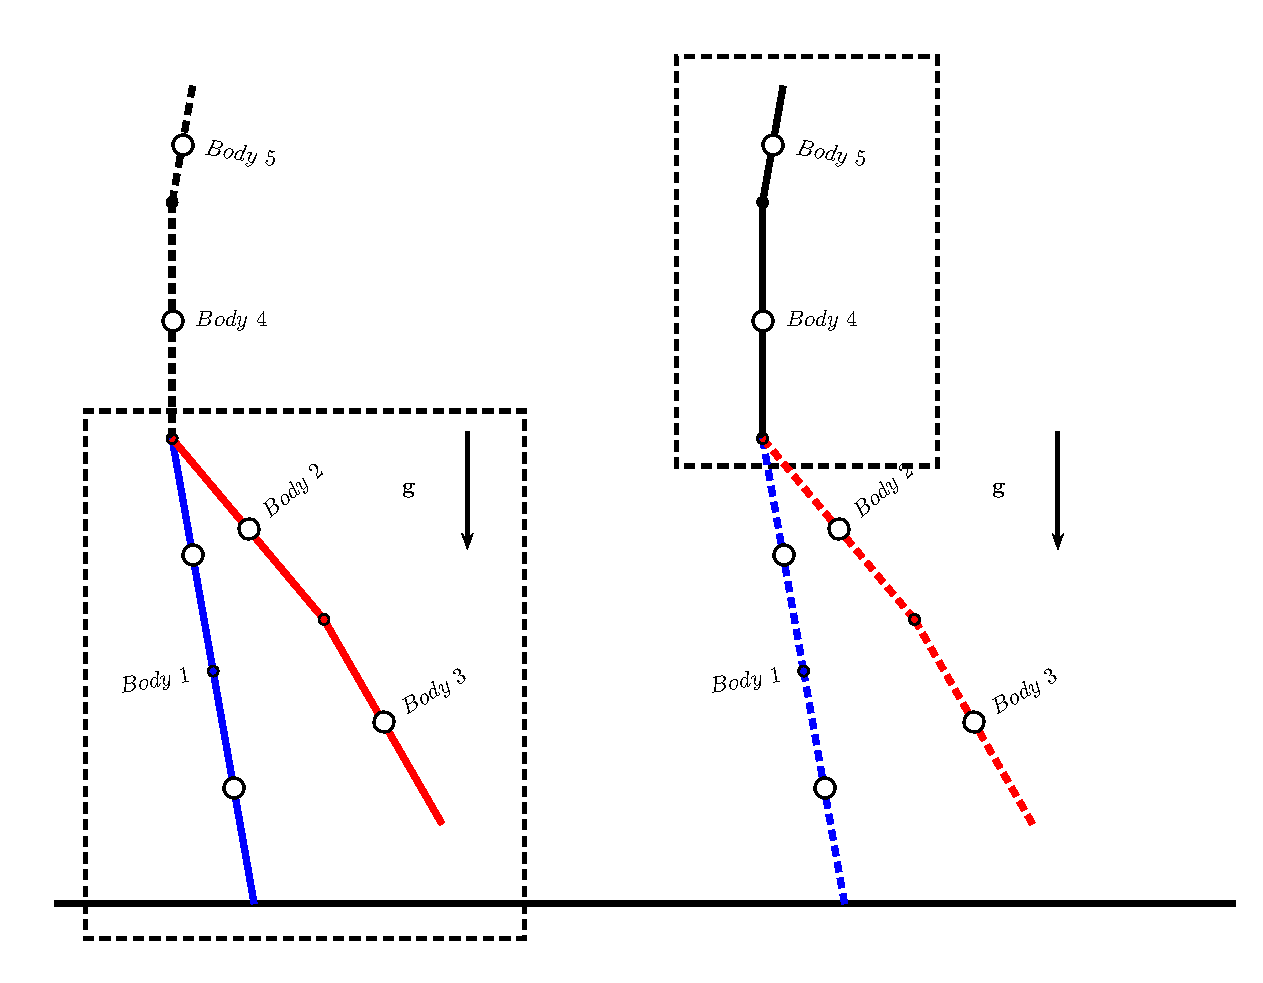
\includegraphics[width=0.7\textwidth]{multilinkCoupled}
    \caption{mechanical coupling}
    \label{fig:mechcouple}
\end{center}
\end{figure}








\subsection*{Torsol And Arm}
using this mechanical coupling method, we can incorporate the arm and torso motion is our dynamic system.
for the torso, the angle is $q_{tor}$,with mass $m_{tor}$ and the distance from the hip is $l_{tor}$
then we can add the torso motion to the knee walker, then the walking motion of the lower body becomes
\begin{equation}
\label{eq:walkcouplewithtorso}
M\ddot{q}+C\dot{q}+N=u-\left[\begin{array}{c}
m_{tor}l_{tor}Lcos(q_{1}-q_{tor})\ddot{q}_{tor}\\
0\\
0\end{array}\right]-\left[\begin{array}{c}
m_{tor}l_{tor}Lsin(q_{1}-q_{tor})\dot{q}_{tor}^{2}\\
0\\
0\end{array}\right]
\end{equation}

by analyzing the equation, if the torque posture kept still, it will have no effects on the lower body walking.
In real life walking, the upper body usually keep straight upward, the coupling input from the upper body is very small.



the torso motion is an inverted pendulum plus some perturbation from the lower body.
\[
m_{tor}l_{tor}^{2}\ddot{q}_{tor}=gm_{tor}l_{tor}sin(q_{tor})-(m_{tor}l_{tor}Lcos(q_{1}-q_{tor})\ddot{q}_{1}-m_{tor}l_{tor}Lsin(q_{1}-q_{tor})\dot{q}_{1}^{2})
\]
by analyzing the torso motion equation, torso motion is unstable in nature, there must be some control applied to maintain its posture.

We are not clear what the kind of controller is applied for maintain the torso posture.
Simple PD controller will work well, but it does not necessary generating believable motion.
An upper body motion is close related to motion purpose and not determined by natural dynamic properties.

For application purpose, maybe it is unnecessary to find a controller for upper body motion.
We can use procedure or other "IK" method to generate upper body motion, and add the dynamic effects to the lower body walking motion.

The motion of arm can be incorporated by following the same principles, it is just another level of complexity.


\section{Boid and Adhoc}

For some sepere and fish, the mechanical system is in chain and involves lots of similar joints.
such system dof can't be neglected or reduced through symmetry and through mechanical coupling.

our propose idea is an adhoc method, we simulate just one dof, other dof following the solution.
since the dynamics is similar, similar strategy will result in similar solution.
such idea have two kinds of application.


The first idea is applying this method for the boid system.
Original boid system is ruled based, but method don't promise stability.
While we using group theory for simulation bold system, if all the agent using the same neural oscillator, they will converge to the same limit circle,
thus guaranty the final motion of the group are in an uniform manner, the different in the agent of modelled by lie group symmetry, different symmetry applied to different agent will result in
difference.
on import symmetry is time offset, which will result in the same motion but of different phases.


In the following example, we have 8 joint,
the form are controlled by the CPG with the same parameters but of different initial condition,
this will result an motion of different phase .


we expend this boid example to model the fish swimming.
The fish is made up 8 links, and each dof is controlled by a neural oscillator.

\begin{figure}[!htbp]
  \begin{center}
      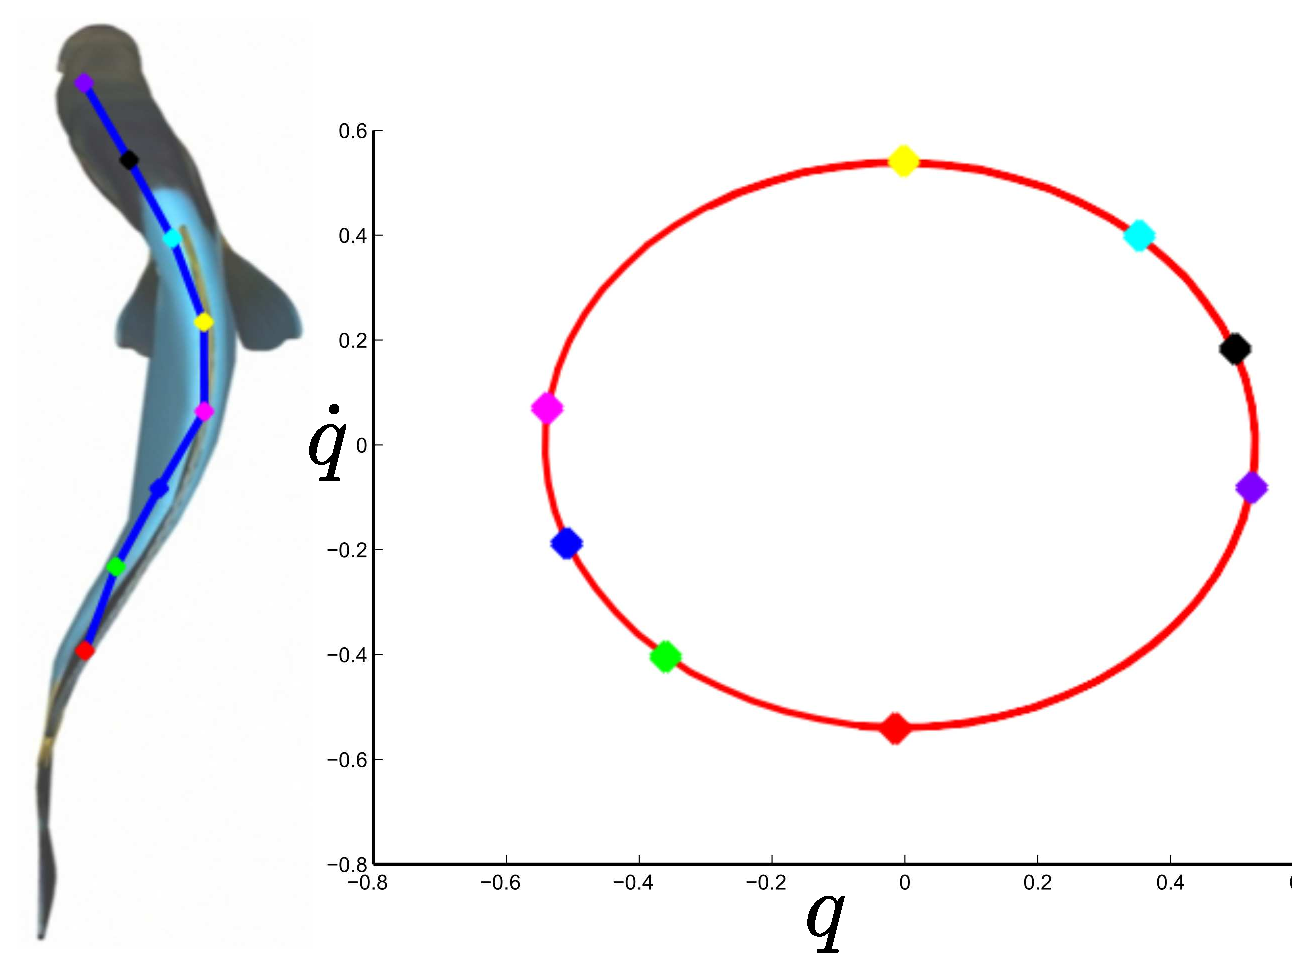
\includegraphics[width=0.5\textwidth]{fish_plot}
    \caption{cPG for Fish}
    \label{fig:fishplot}
\end{center}
\end{figure}

\begin{figure}[!htbp]
  \begin{center}
      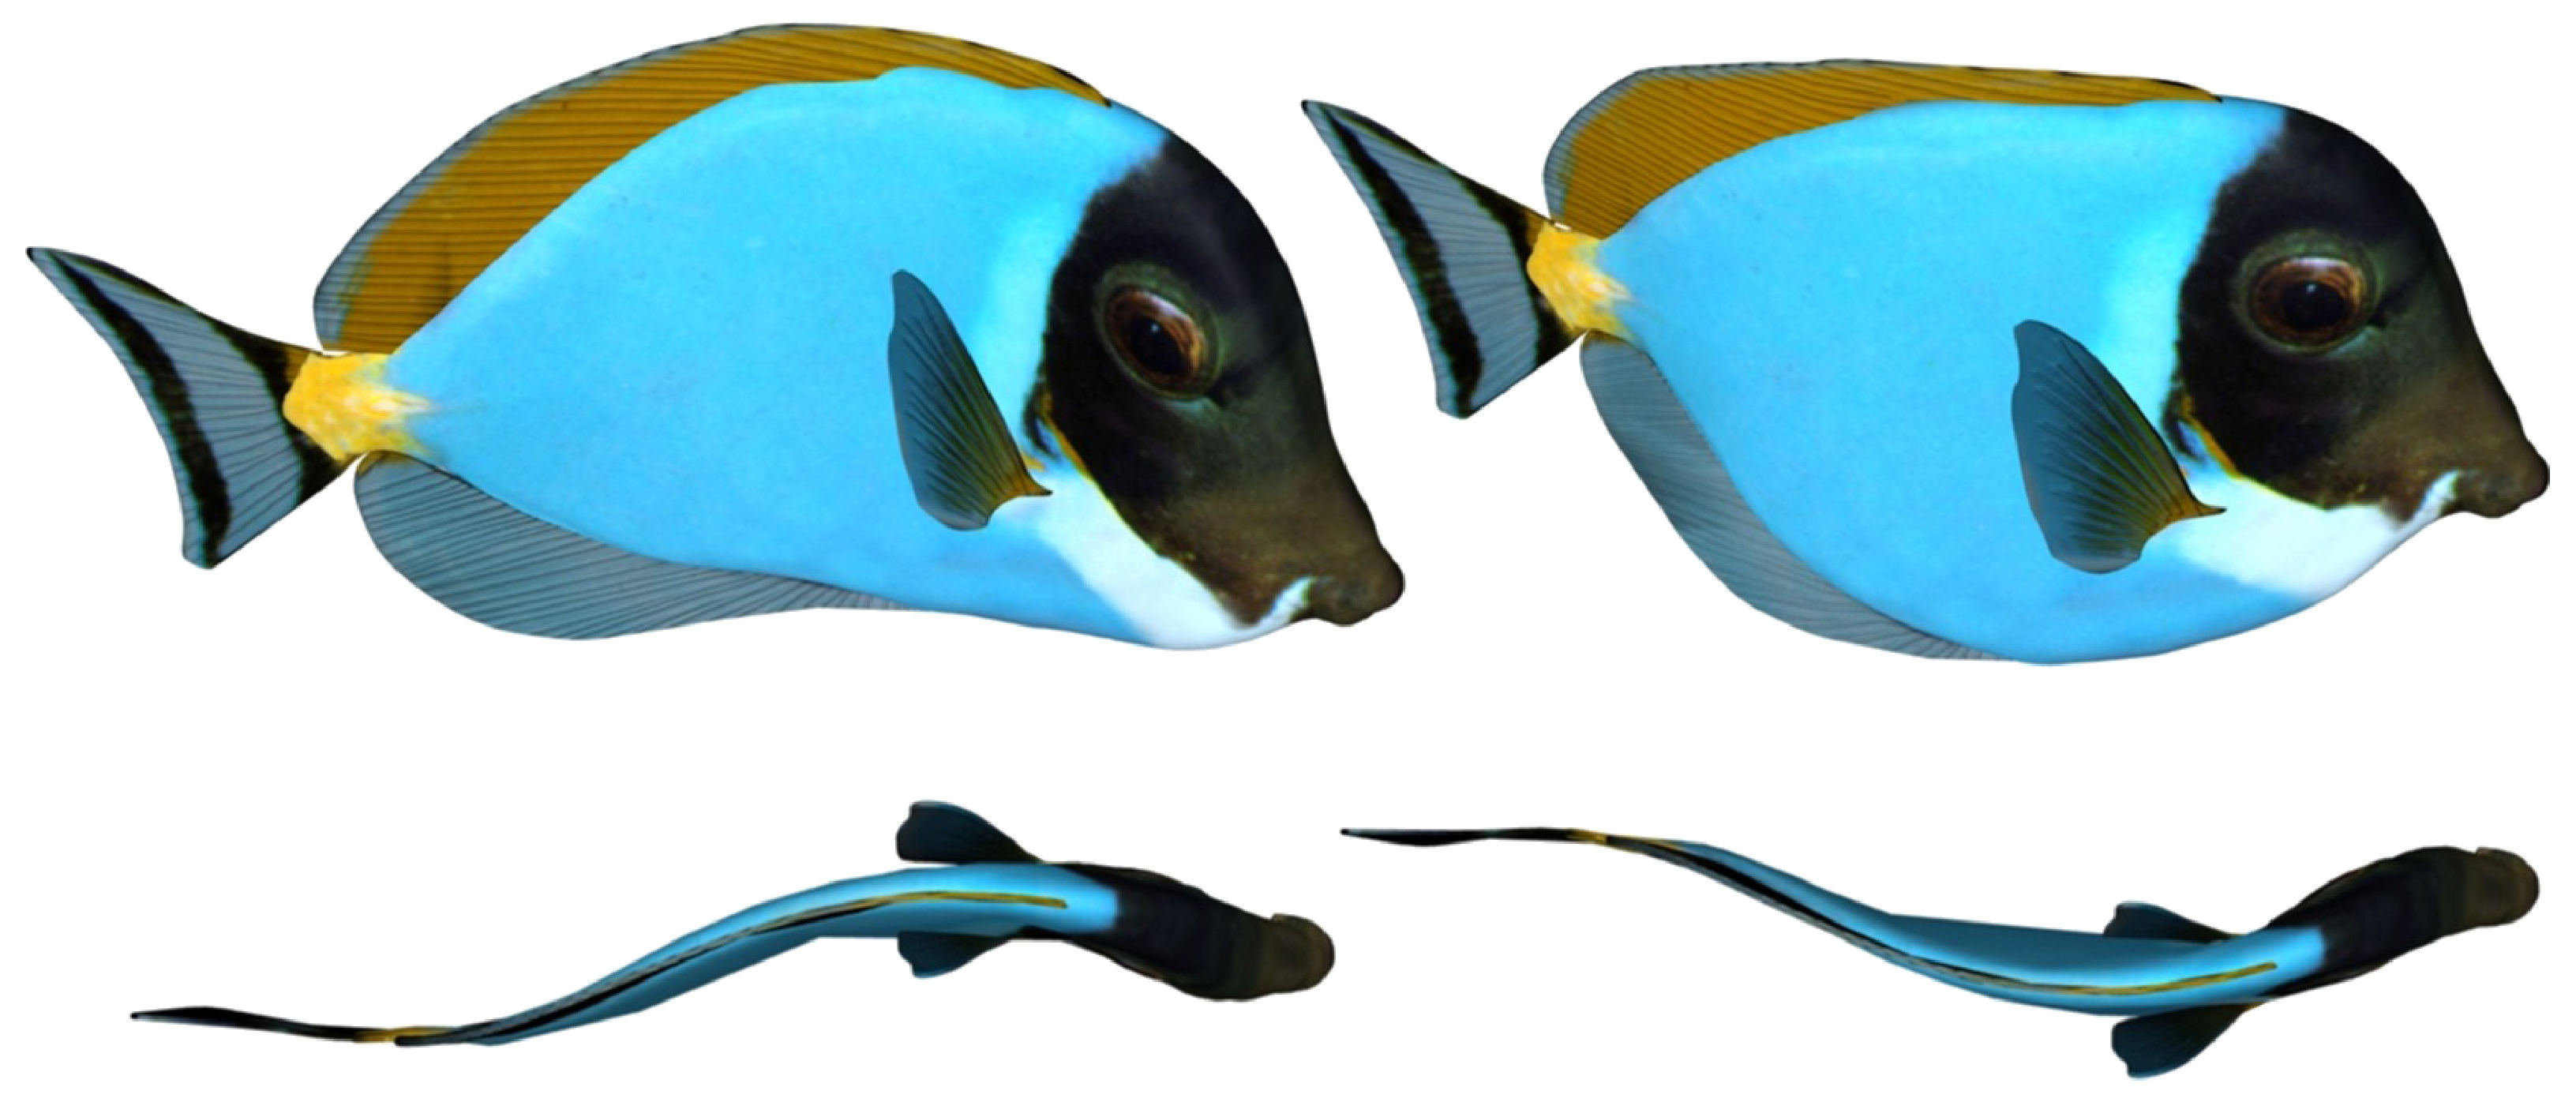
\includegraphics[width=0.5\textwidth]{fish_swimming}
    \caption{Swimming Motion by our method}
    \label{fig:fishswimming}
\end{center}
\end{figure}




the same symmetry is applied to the 8 neural oscillator, then it will modify the system in an unified manner.

as show in picture



\section{From Low Dimention To High Dimension}

For computer animation, even we can get high dimensional results, maybe it does not meet the animators needs.
simulation result in motion can be treat as a reference, rather than put into result in deformation.

we can describe the motion procedures, and using mechanical simulation a low dof to drive the high dimensional motion.
in the following example,
we describe the jumping motion in an procedure method,
and bouncing ball is used to drive the motion.


also we can using the low dimension data as a key word to search motion capture data.
which will give us more realistic motion results.



